\documentclass[draftclsnofoot,onecolumn,journal,letterpaper,compsoc,10pt]{IEEEtran}
\usepackage{geometry}
\usepackage{setspace}
\usepackage{titling}
\usepackage{pdfpages}

\geometry{letterpaper, margin=.75in}
\singlespace

\begin{document}

\title{Project Update: Fall\\\large CS 461 Fall 2018\\Group 19 BrewHops: Ninkasi Brewing, Automating the brewing process}
\author{
    Brennan Douglas \\
    \texttt{douglbre@oregonstate.edu} \\
    \and
    Dan Van Horn \\
    \texttt{vanhornd@oregonstate.edu} \\
    \and
    Henry Peterson \\
    \texttt{peterhen@oregonstate.edu} \\
    \and
    Bailey Singleton \\
    \texttt{singletb@oregonstate.edu} \\
}
\date{November 27th, 2018}

\begin{titlingpage}
    \maketitle
    \begin{abstract}
    	During the beer brewing process there are many variables that need to be tested and tracked. This helps determine when the beer is ready and how it compares to other batches. Ninkasi --- a brewery in Eugene, Oregon --- is using a single large excel spreadsheet to track and store all their information. As they have grown, this has become increasingly unwieldy. There is already the beginning of a solution which includes a small set of applications designed to manage this data automatically while allowing for editing and visualization. This system will manage brewing data and user permissions to reduce the possibility for human error.  This document summaries the work done towards this project.  This includes a week by week account of what we accomplished and had issues with.
    \end{abstract}
    \pagebreak
    \tableofcontents
\end{titlingpage}

\section{Recap}
The main goal of this project is to have a system that will streamline the process of recording, storing, and viewing data gathered during the beer brewing process. A previous group has already implemented a portion of this system, making it our task to take it to a production-ready state. Their contributions consist of setting up the server, designing an initial database, creating a user-interface, and connecting them all using docker containers. Our plan includes implementing testing, fixing bugs in the behaviour and style, adding new features requested by the client, and finally creating a robust deployment process.


\section{Progress}
Over the course of the term we have written about and designed this project extensively. The pros and cons of the current system were taken into account when deciding future actions as well as requests from the client. The GitHub project board reflects these decisions and some development under the Maintenance epic has already taken place.

We have updated the use of Docker in the project by containerizing each of our applications as opposed to the database only. Converting the project to Typescript is in progress with the back-end conversion completed and the front-end under development. Finally, we are strongly emphasizing the use of testing frameworks in the project. The back-end already has integration testing implemented, but we believe that a full suite of unit test is required before significant feature development can take place.

\section{Problem Summary}
    Problems were few and far between this term. During the initial starting phase of the project, we thought that we were not going to be put on the Ninkasi team, as it was not showing on the project list. After clearing that up and talking to our client, we got approved on the project. 
    A roadblock we initially ran into was getting familiar with the code, as is usual when taking over someone else's project. It took time and research to figure out the software that was being used, and turned out to be a great learning opportunity.
    Setting up a meeting time that worked for our entire group turned out to be a formidable challenge. With different schedules and work hours, it became clear that we needed to establish a day in the week when we could all put aside some time to work on the important aspects of our assignments.


\section{Retrospective}

\vspace{2mm}
\begin{center}
    \begin{tabular}{|p{0.3\linewidth}|p{0.3\linewidth}|p{0.3\linewidth}|}
        \hline Positives & Deltas & Actions \\
        \hline
            {\bf Brennan:}\newline
            Efficient planning and execution on the documentation.  Allowed us to work at our own paces and regroup at the due date to compose all of our pieces.  Also, got an early start to the development by playing with the pre-existing code. Got most all of documentation complete for the year. &
            {\bf Brennan:}\newline
            Communication with Joe, our advisor, could have been more continuous.  We only met once and didn't check in with him when he didn't respond to the documents he sent us. &
            {\bf Brennan:}\newline
            More emails should be sent to Joe during the development of the application letting him know of our status and any issues we have completed.  We will remain vigilant to confirm that we receive a response from him by emailing him back if he has not replied within two days of the email being sent. \\
        \hline
            {\bf Dan:}\newline
            Teamwork on design and documentation has been top-notch. We've been able to assign tasks in such a way that we do not block each others progress. We've planned the preliminary development of the Maintenance epic and some work is currently underway. &
            {\bf Dan:}\newline
            We need to keep a more consistent line of communication with our client. Team communication is good but we could stand to improve in updating each other more frequently on our progress. &
            {\bf Dan:}\newline
            We will adhere to our GitHub project board as the single source of truth for the progress of our application. We will also be more vigilant about receiving client feedback.  \\
        \hline
            {\bf Henry:}\newline
                I was pleased with the promptness of our team. We met with our client quickly, start on assignments early, and quickly figure out who needs to do what. I've been in too many projects where I am the primary motivator, and it is nice to have it more consistent with this group. &
            {\bf Henry:}\newline
                We have had relatively infrequent contact with our client. Part of this come from having some of the project already implemented; I think many of our questions are answered by looking at the structure of the code or talking to the previous group. &
            {\bf Henry:}\newline
                We should have bi-weekly check ins with the client stating the work we have done along with any questions we may have. The will keep everyone more in the loop on what is happening. I also think that this will become increasingly valuable as we move into the implementation section of the project. \\
        \hline
            {\bf Bailey:}\newline
            Our team meshes well together, and we are very proactive to get things done ahead of time. This lends well to a project with strict deadlines, and lessens the stress when those deadlines come around. &
            {\bf Bailey:}\newline
            Communication on who was doing what could have been a bit better. Sometimes it was hard to know if something was going to get done, only to find out that it had been taken care of a while ago. &
            {\bf Bailey:}\newline
            More communication will help us with next terms' goals. If we can improve upon filling each other in on who has done what, we will exceed expectations. We are eager to dive into the code, so it will not be a problem for getting things done. \\
        \hline
    \end{tabular}
\end{center}

\section{Weekly Summaries}

    \subsection{Week 1}
    We attended the first few lectures of class and began learning what this year would look like.  We accustomed ourselves to what would be expected of us throughout the upcoming terms.

    \subsection{Week 2}
    We had a problem at the beginning of the term as our project was not on the project list.  We had been communicating with our advisor for months ahead of time and had already informed Kristin of our project and plans.  However when the list was released it was nowhere to be found.  So, with a few quite emails and forwarding an old email chain to prove we had been planning this since summer we were able to get the project confirmed and on the list.
    
    \subsection{Week 3}
    We were assigned our project/team and set up communication channels.  These included a slack work space and email sharing.  We planned a meeting with our advisor the following week to go over the list of requirements that we had from a meeting with him in the summer.
    
    \subsection{Week 4}
    We attending our group meeting with Joe and he was thrilled at our list of requirements.  This allowed us to easily move forward with our project goals as we had a complete list of what we needed to accomplish for the project to be complete.
    
    We used the information from this meeting to write our individual problem statements for our project.  The finalized list allowed us to cleanly lay out what the scope of the problem was.
    
    
    \subsection{Week 5}
    We began work on the requirements document by sitting down as a team and creating a list of Epics and Stories to go within the Epics.  We then created an outline for the requirements document using these and split up the work from there.  We all completed our sections and then met back together to create the gantt chart.  Once that was complete we submitted our requirements document and emailed it off to our advisor to get his thoughts.
    
    From there we created our tech review divisions and assigned them to group members so we could begin working on it when we liked.  We spent the last half of the week working on our individual tech reviews.
    
    
    \subsection{Week 6}
    We submitted our first drafts of the tech reviews.  Then in class during the week we did peer reviewing of different students tech reviews.  We used this feedback to review our tech review draft into the final submission.
    
    
    \subsection{Week 7}
    We all finished work on our final tech review draft and submitted them.  Not much else went on this week.
    
    
    \subsection{Week 8}
    We set the outline for the design document during our weekly group meeting and split up the work along the same lines as the tech review.  Event though we all agree that we will all be able to work on all levels of the application it made the most sense to keep the roles as they were for the documentation phase.
    
    We then started our first bit of work on the actual development of the application.  We created our project board on GitHub and laid out tasks for our iteration zero.  This involves getting the existing code running and setting up the new docker development environment that we wish to work in.
    
    
    \subsection{Week 9}
    We started to work on the design document and created a shared Google slides for our project update video that we need to complete.  We made plans to film the video during our weekly meeting on week 10.  This is when the outline of the project update was also originally made.  There was no group meeting this week due to thanksgiving break and the team not being in town to attend.
    
    Work was also begun on the TypeScript conversion of the application.  This was the start of the long task to re-factor the existing JavaScript code into TypeScript.
    
    
    \subsection{Week 10}
    We completed the design document in the niche of time (submitting our final draft 1 minute before it was due).  After that the PowerPoint slides for the progress report video were finished.  Once completed we all met and ran through voicing over each of the slides.  This involved recording audio clips rotated through the group members on a per slide basis.  The audio clips were then edited over pictures of the slides and the video was rendered.
    
    After the video was complete the progress report was finished (having been already started over thanksgiving break).  Once we completed all of the documents we sent them off with instructions to Joe, our advisor, for him to go through the client verification process.
    
    
\section{Looking Forward}
We have no planned work that we are going to complete over winter break.  As soon as winter term starts we are going to move ahead on understanding the existing code.  While we are doing this we will be writing unit tests for the code so that when we start changing things and adding features we know if accidentally broke existing code.  From there we will begin implementing each of the features in line with our gantt chart (appended to this document) starting from winter term.

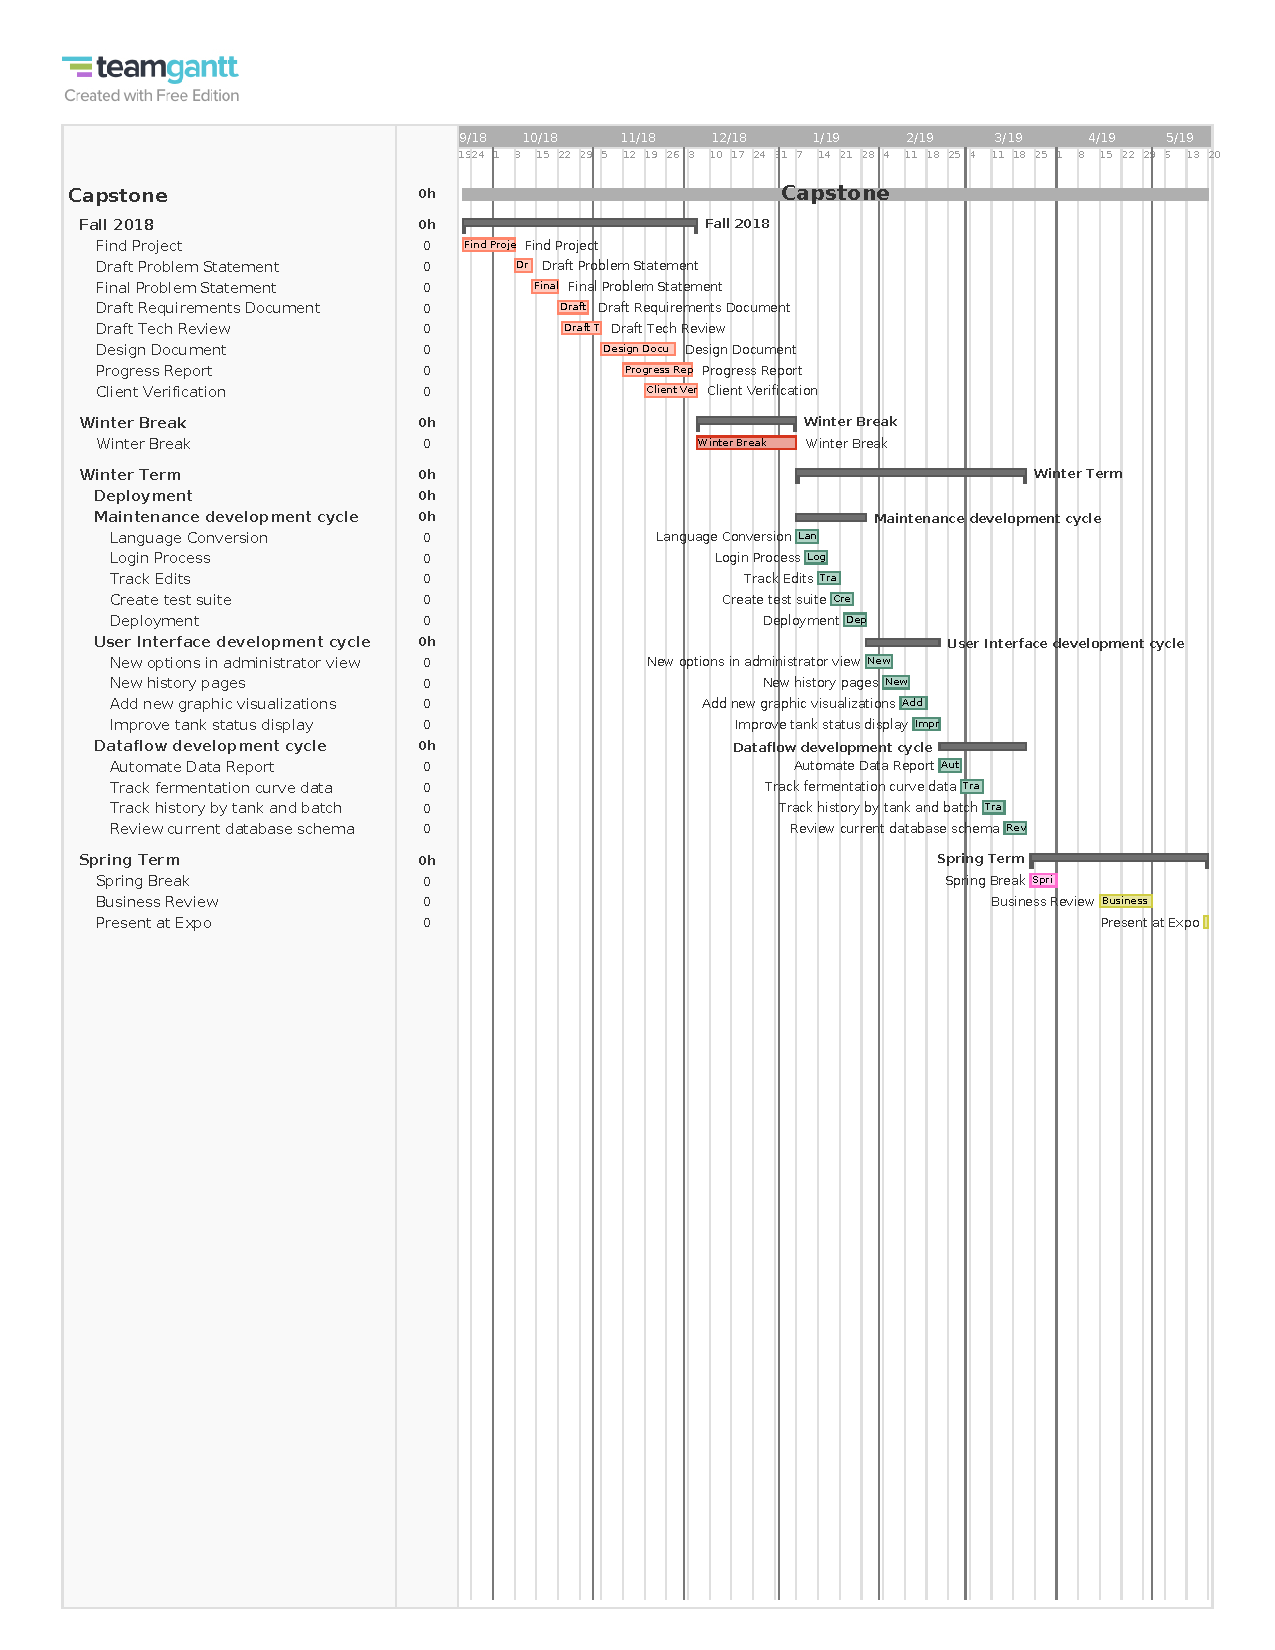
\includepdf[pages=1]{Capstone.pdf}

\end{document}
